%\documentclass{standalone}
%\usepackage{standalone}
%\usepackage[custom,pgfkeys]{ati}
%\begin{document}
\begin{atiTask}[
  title = Kuppelkatastrophe,
  %call = Zusatzaufgabe,
]

Gegeben sei eine halbkugelförmige Kuppel mit Radius $R$, deren Mittelpunkt im Ursprung des Koordinatensystems liege. Die Kuppel sei mit einem giftigen Gas gefüllt. Der bösartige Simon Bar Sinister sorgt dafür, dass die gesamte Kuppel kurz durchlässig wird, so dass eine winzige Menge Gas entweichen kann. Die Dichte des Gases $\rho=D_0$ ist als konstant anzunehmen. Außerhalb der Kuppel wehe der Wind mit der Geschwindigkeit 
\[
\vec{v}(x,y,z)=(5kx+py^2)\vec{i} +ky \vec{j}\quad p,k=\text{const}.
\]  

\begin{atiSubtasks}
\item Berechnen Sie den Massenstrom der austretenden Chemikalie, indem Sie das Oberflächeintegral über die Impulsdichte bilden.
\item Verifizieren Sie den \textsc{Gauss}schen Satz, indem Sie den Massenstrom noch einmal über ein Volumenintegral berechnen.
\item Führen Sie für das Ergebnis eine Einheitenbetrachtung durch. 
\end{atiSubtasks}
  
\end{atiTask}

\begin{atiSolution}
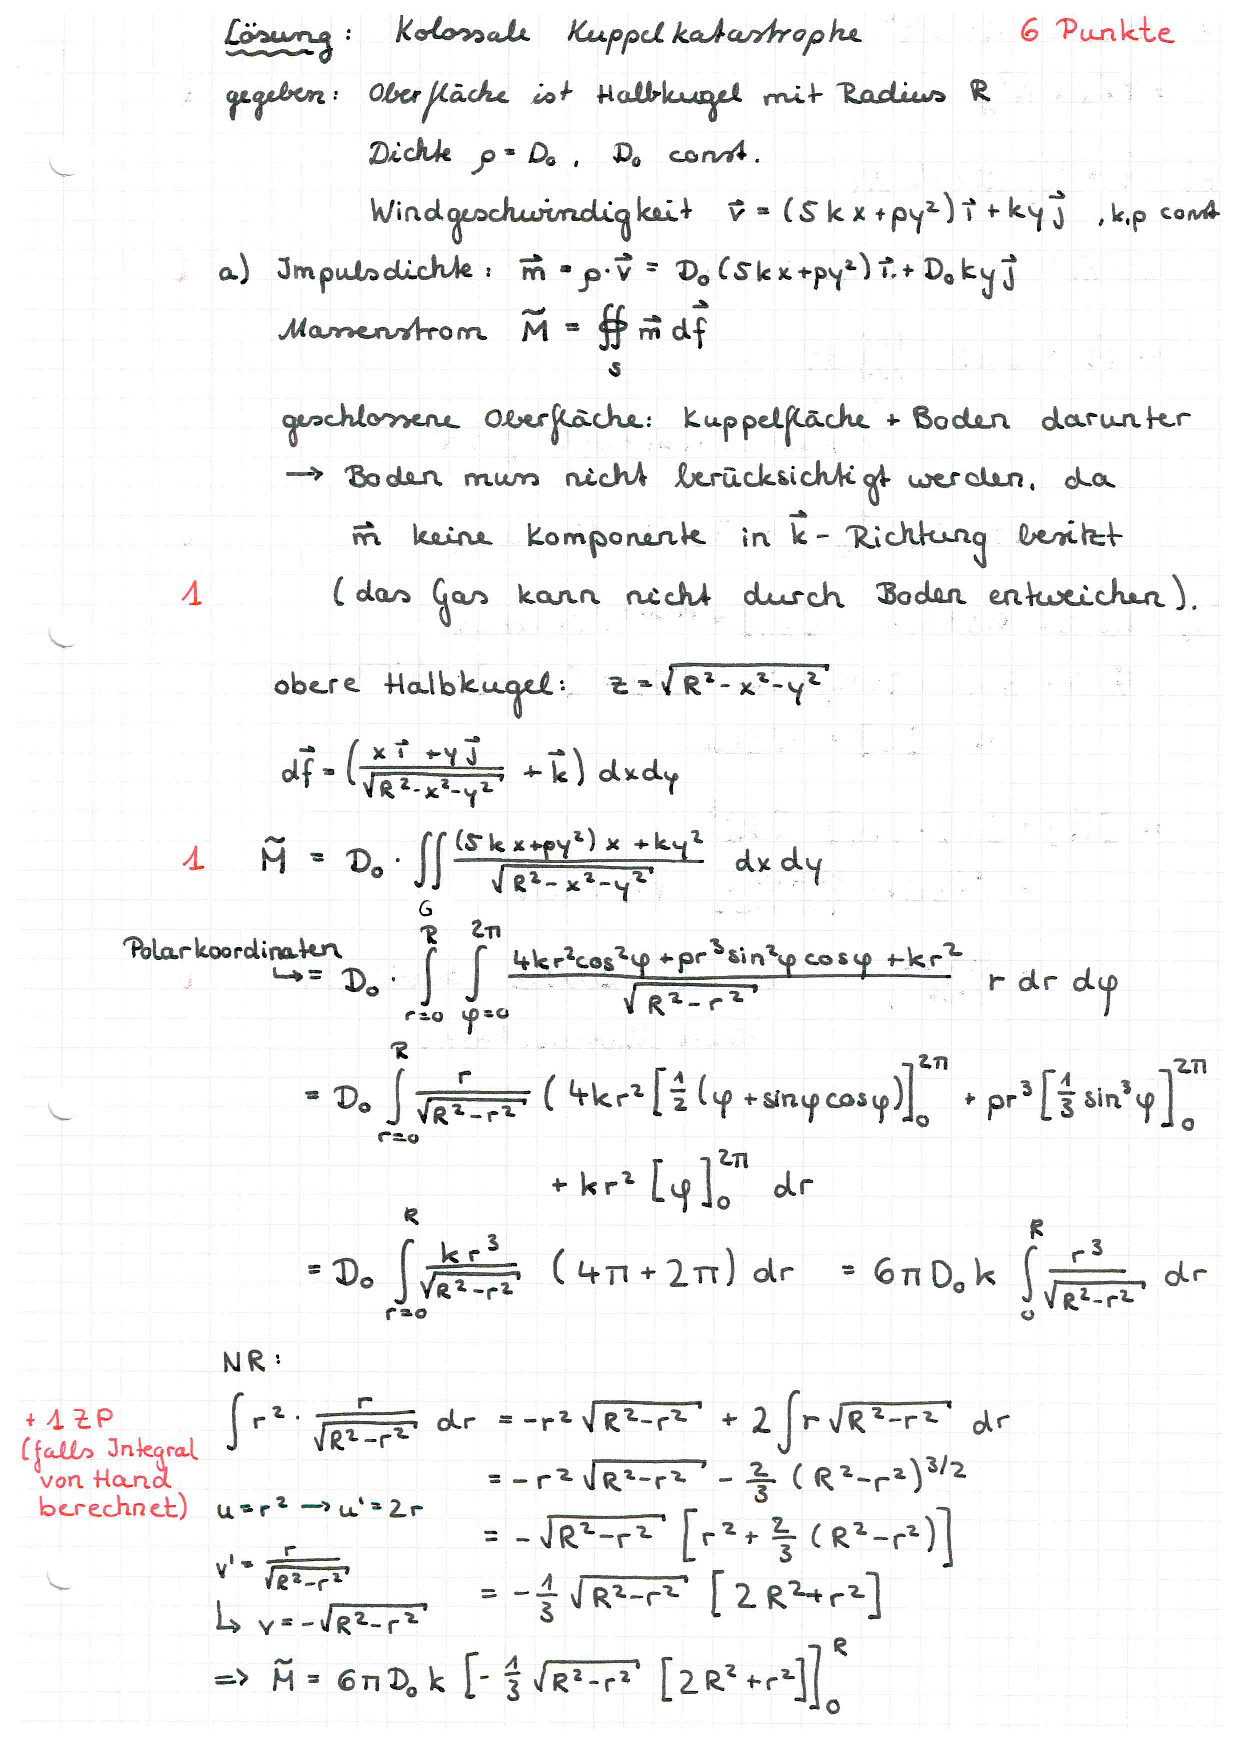
\includepdf[pages=-]{solution-kuppelkatastrophe.pdf}
\end{atiSolution}

%\end{document}